% Particle-decay cascade regression with a child-local grow' override.
\documentclass[border=2pt]{standalone}
\usepackage{tikz}
\usetikzlibrary{trees}

\tikzset{
  particle/.style={draw,circle,minimum size=10mm,inner sep=1pt,fill=blue!10},
  product/.style={draw,rounded corners=2pt,minimum width=11mm,minimum height=7mm,inner sep=1pt},
  every edge from parent/.style={draw,thick,-stealth}
}

\begin{document}
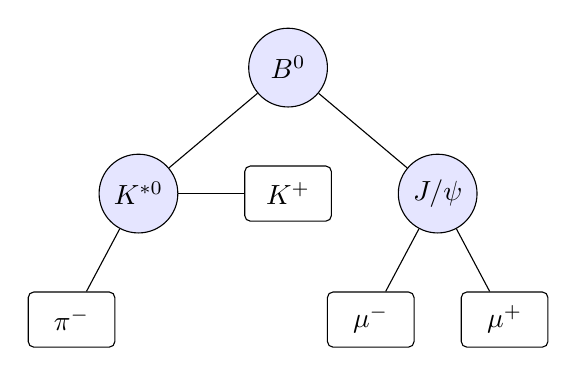
\begin{tikzpicture}[
  grow'=down,
  level distance=16mm,
  level 1/.style={sibling distance=38mm},
  level 2/.style={sibling distance=17mm}
]
  \node[particle] {$B^0$}
    child {
      node[particle] {$J/\psi$}
      child {node[product] {$\mu^+$}}
      child {node[product] {$\mu^-$}}
    }
    child {
      node[particle] {$K^{*0}$}
      child[grow'=right,level distance=19mm] {node[product] {$K^+$}}
      child {node[product] {$\pi^-$}}
    };
\end{tikzpicture}
\end{document}
